\documentclass[11pt]{article}
\usepackage[a4paper,margin=2.4cm]{geometry}
\usepackage[T1]{fontenc}
\usepackage{lmodern}
\usepackage{amsmath,amssymb}
\usepackage{graphicx}
\usepackage{booktabs}
\usepackage{microtype}
\usepackage[hidelinks]{hyperref}
\usepackage[labelfont=bf,font=small]{caption}
\usepackage{authblk}
\usepackage{natbib}
\bibliographystyle{unsrtnat}
\usepackage{xcolor}
\usepackage{titlesec}
\titleformat{\section}{\normalfont\large\bfseries}{\thesection}{0.7em}{}
\titleformat{\subsection}{\normalfont\normalsize\bfseries}{\thesubsection}{0.6em}{}
\setlength{\parskip}{0.35em}
\renewcommand{\arraystretch}{1.12}

%%% ---------------------------------------------------------------------------
%%% All reported numbers are defined here and nowhere else, so that the text and
%%% the analysis outputs cannot drift apart. Regenerated by paper/update_numbers.py
%%% ---------------------------------------------------------------------------
% generated by paper/update_numbers.py -- do not edit by hand
\newcommand{\NinsTot}{95,184}
\newcommand{\NdelTot}{46,660}
\newcommand{\Nposdel}{35,877}
\newcommand{\Ndom}{748}
\newcommand{\Nposins}{34,113}
\newcommand{\Ndesign}{57}
\newcommand{\NresContrast}{18}
\newcommand{\Offset}{0.315}
\newcommand{\OffsetLo}{0.284}
\newcommand{\OffsetHi}{0.345}
\newcommand{\NoffDom}{743}
\newcommand{\Slope}{-0.68}
\newcommand{\SlopeLo}{-0.88}
\newcommand{\SlopeHi}{-0.48}
\newcommand{\Intercept}{0.86}
\newcommand{\SlopeNoGly}{-0.58}
\newcommand{\SlopeNoGlyLo}{-0.81}
\newcommand{\SlopeNoGlyHi}{-0.37}
\newcommand{\SlopeStrand}{-0.49}
\newcommand{\SlopeStrandLo}{-0.79}
\newcommand{\SlopeStrandHi}{-0.16}
\newcommand{\RhoStrand}{-0.52}
\newcommand{\RhoHE}{-0.33}
\newcommand{\RhoHElo}{-0.47}
\newcommand{\RhoHEhi}{0.04}
\newcommand{\PooledR}{0.383}
\newcommand{\PerDomR}{0.514}
\newcommand{\SlopeNaive}{0.712}
\newcommand{\SlopeIV}{0.870}
\newcommand{\SlopeIVLo}{0.834}
\newcommand{\SlopeIVHi}{0.906}
\newcommand{\FdelInter}{8.77}
\newcommand{\PdelInter}{3.8\times10^{-46}}
\newcommand{\FdelPerm}{1.36}
\newcommand{\PdelPerm}{0.08}
\newcommand{\RhoPace}{-0.64}
\newcommand{\RhoPaceLo}{-0.74}
\newcommand{\RhoPaceHi}{-0.41}
\newcommand{\RhoVol}{0.25}
\newcommand{\RhoKD}{-0.17}
\newcommand{\PartialPaceVol}{-0.61}
\newcommand{\PartialVolPace}{0.05}
\newcommand{\PartialPaceHydro}{-0.65}
\newcommand{\AlaHL}{0.066}
\newcommand{\AlaHLlo}{0.022}
\newcommand{\AlaHLhi}{0.110}
\newcommand{\GlyHL}{0.374}
\newcommand{\GlyHLlo}{0.328}
\newcommand{\GlyHLhi}{0.422}
\newcommand{\AlaEL}{-0.228}
\newcommand{\AlaELlo}{-0.278}
\newcommand{\AlaELhi}{-0.177}
\newcommand{\GlyEL}{-0.003}
\newcommand{\GlyELlo}{-0.052}
\newcommand{\GlyELhi}{0.046}
\newcommand{\GateH}{0.309}
\newcommand{\GateE}{0.258}
\newcommand{\GateL}{-0.017}
\newcommand{\DesAlaHL}{-0.126}
\newcommand{\DesGlyHL}{-0.010}
\newcommand{\DesStrandHelix}{-0.024}
\newcommand{\DesStrandHelixLo}{-0.111}
\newcommand{\DesStrandHelixHi}{0.067}
\newcommand{\PredAdd}{0.211}
\newcommand{\PredInter}{0.216}
\newcommand{\PredGain}{0.006}
\newcommand{\PredGainLo}{0.001}
\newcommand{\PredGainHi}{0.011}
\newcommand{\PredNdom}{746}
\newcommand{\PredImproved}{52\%}
\newcommand{\PredGeomAdd}{0.379}
\newcommand{\PredGeomInt}{0.368}
\newcommand{\HelMidEnd}{0.481}
\newcommand{\HelMidEndLo}{0.387}
\newcommand{\HelMidEndHi}{0.575}
\newcommand{\NhelDom}{223}
\newcommand{\RhoLoop}{-0.023}
\newcommand{\RhoLoopLo}{-0.058}
\newcommand{\RhoLoopHi}{0.012}
\newcommand{\StrandHelix}{-0.478}
\newcommand{\StrandHelixLo}{-0.661}
\newcommand{\StrandHelixHi}{-0.288}
\newcommand{\SSagree}{80.1\%}
\newcommand{\NumberMatch}{1.000}
\newcommand{\NumberChecks}{36,047}
\newcommand{\PooledPerm}{$-0.169$ $[-0.272, -0.057]$}
\newcommand{\WithinPerm}{0.0009}
\newcommand{\WithinPermSD}{0.060}


\title{\bfseries The secondary-structure dependence of indel cost is a property of the
residue, not of the indel}

\author[1]{Armin Ziaei}
\author[2]{Sheida Farrokhi}
\affil[1]{Independent Researcher. Correspondence: \texttt{armin.ziaei.tech@gmail.com}}
\affil[2]{Independent Researcher. \texttt{sheyda.farrokhi.id@gmail.com}}
\date{\today}

\begin{document}
\maketitle

\begin{abstract}
\noindent
Single-residue insertions and deletions are the second most common class of protein-coding
variant, and their effects are usually summarised by secondary-structure class: helices tolerate
indels poorly, strands worse still, loops best. Using the mega-scale folding-stability
measurements of \citet{tsuboyama2023} we compare insertions and deletions \emph{at the same
position in the same protein} across \Nposdel{} single deletions and \Nposins{} positions carrying
both an alanine and a glycine insertion, across \Ndom{} domains --- \NNatDom{} natural and
\NDesDom{} designed, which we analyse both together and apart. We find that the
structure--class summary is not well defined, because the structural dependence belongs to the
residue involved rather than to the indel. For deletions, where all twenty residues occur,
residue identity interacts with structure class at $F = \FdelInter{}$, $p = \PdelInter{}$ after
domain fixed effects, burial and volume, and the interaction is ordered: the extra cost of
deleting a residue from a helix rather than a loop tracks that residue's helix propensity
($\rho = \RhoPace{}$, bootstrap CI over domains $[\RhoPaceLo{}, \RhoPaceHi{}]$), and not its
volume ($\rho = \RhoVol{}$) or hydropathy ($\rho = \RhoKD{}$). The ordering replicates separately
in the natural domains ($\rho = \RhoNat{}$ $[\RhoNatLo{}, \RhoNatHi{}]$) and in the designed ones
($\RhoDes{}$ $[\RhoDesLo{}, \RhoDesHi{}]$), which share no evolutionary history with them, and it
survives replacing our secondary-structure assignment with the one deposited with the
experimental structures, though weakened ($\rho = \SensDep{}$ $[\SensDepLo{}, \SensDepHi{}]$). For insertions, switching the
inserted residue between alanine and glycine moves the helix--loop contrast by about
0.3 kcal\,mol$^{-1}$ (\AlaHL{} to \GlyHL{}) and the strand--loop contrast by about 0.2
(\AlaEL{} to \GlyEL{}). The interaction is nonetheless too small to improve
leave-one-domain-out prediction over an additive model once simple geometric features are
included, which bounds how much practical weight it carries. We also report three negative results: the
helix accommodation energies measured crystallographically in T4 lysozyme do not transfer to this
scale, indel cost does not depend on distance to the nearest loop, and an apparent within-protein
advantage of strands over helices fails to replicate in the designed set.
\end{abstract}

\section{Introduction}

Insertions and deletions of one or a few residues are the second most common class of
protein-coding variant after substitutions, and the least well understood. Substitutions have
been characterised at scale for a decade; indels have not, because they change the length of the
chain and therefore break the one-to-one mapping between wild-type and variant positions on which
most analysis pipelines and most variant-effect predictors depend.

Systematic measurements exist for a handful of proteins --- single alanine and glycine insertions
in staphylococcal nuclease \citep{sondek1990,sondek1992}, a complete insertion and deletion scan
of TEM-1 $\beta$-lactamase \citep{gonzalez2019}, random deletions in GFP \citep{arpino2014},
insertion and deletion libraries in Kir2.1 \citep{macdonald2023} and in an enterovirus proteome
\citep{bakhache2025}, and indel libraries for directed evolution \citep{emond2020,hallet1997} ---
and, at scale, in the mega-scale stability measurements of \citet{tsuboyama2023} and the deep
indel mutagenesis of \citet{topolska2025}.

The summaries that do exist are organised by secondary structure. \citet{topolska2025} measured
indel effects across nine protein domains and re-analysed the mega-scale stability data of
\citet{tsuboyama2023}, reporting that loops are more tolerant than structured elements and that
$\beta$-strands are slightly less tolerant than $\alpha$-helices, though they note the differences
are small. \citet{macdonald2023} reached a similar conclusion for Kir2.1, and
\citet{larsenledet2025} report for human DHFR that deletions are more detrimental in strands than
in helices while insertions are not. \citet{goldman2025} gave the
sharpest mechanistic account: helices are especially sensitive to indels because their
$3.6$-residue periodicity means a length-altering edit shifts the register of everything
downstream, so that ``their periodicity renders size-altering mutations more deleterious compared
to size-conservative mutations''. On this account the structural penalty is a property of the
\emph{edit} --- of what it does to the backbone --- and it should be largely the same whichever
residue is involved.

That prediction is testable, because the mega-scale data contain both halves of the comparison.
Deletions remove the wild-type residue, so all twenty amino acids are represented; insertions in
these libraries are alanine or glycine, so the same position can be probed with two residues that
differ by a single methyl group but by a full kcal\,mol$^{-1}$ of helix propensity
\citep{pace1998}. If the structural penalty belongs to the edit, neither comparison should show
much residue dependence. If it belongs to the residue, both should.

We find the latter, and the effect is large enough to change how the field's summary statements
should be written. We also report what did not survive: two framings that looked strong and were
withdrawn on their own controls, and three published claims that do not transfer to this scale.

\section{Results}

\subsection{A deletion costs more than an insertion at the same position}

\begin{figure}[t]
\centering
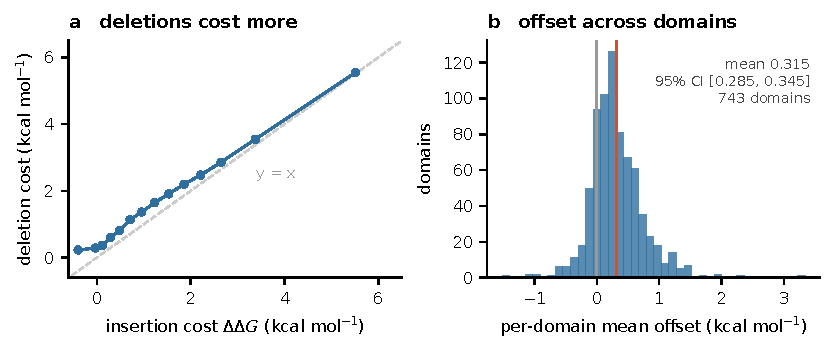
\includegraphics[width=0.92\textwidth]{fig1.pdf}
\caption{\textbf{Deletions cost more than insertions at the same position.}
\textbf{(a)} Mean deletion cost against mean alanine insertion cost, in twelve bins of equal
size; the dashed line is $y=x$. The relationship is close to proportional but sits above the
diagonal across the range. \textbf{(b)} Distribution over proteins of the within-protein mean
offset between the two edits. Each protein contributes one value, and the red line is the mean.}
\label{fig:fig1}
\end{figure}

Throughout, cost is defined as $\Delta\Delta G = \Delta G_{\mathrm{wt}} - \Delta G_{\mathrm{var}}$
in kcal\,mol$^{-1}$, so that a larger cost is more destabilising, and every class comparison is
computed within each protein and then averaged over proteins (Methods). Across \NoffDom{} domains
the mean within-protein offset between a deletion and an alanine insertion at the same position is
\Offset{} kcal\,mol$^{-1}$ (95\% CI $[\OffsetLo{}, \OffsetHi{}]$; Figure~\ref{fig:fig1}). That
deletions are the more damaging edit on average is already known qualitatively
\citep{topolska2025,larsenledet2025}; the paired magnitude is not.

The relationship between the two edits is close to proportional but not quite: regressing deletion
on insertion cost within each protein gives a slope of \SlopeNaive{}, which rises to \SlopeIV{}
$[\SlopeIVLo{}, \SlopeIVHi{}]$ once measurement error on the predictor is instrumented with the
second, independent insertion at the same position. The deletion penalty is roughly twice as large
at tolerant positions as at intolerant ones, but it does not vanish
(Supplementary Figure~S1).

\subsection{Deletions: the structural penalty is ordered by helix propensity}

\begin{figure}[t]
\centering
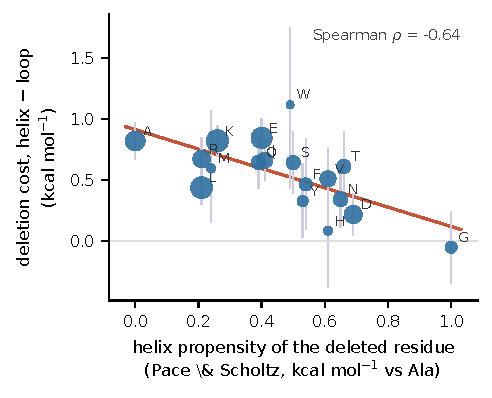
\includegraphics[width=0.62\textwidth]{fig2.pdf}
\caption{\textbf{The extra cost of deleting a residue from a helix depends on which residue it is.}
Each point is one amino acid; the vertical axis is the mean deletion cost at helix positions minus
that at loop positions, paired within each protein and then averaged over proteins, with bootstrap
intervals over proteins. The horizontal axis is the experimental helix propensity of
\citet{pace1998}, a penalty in kcal\,mol$^{-1}$ relative to alanine, so that larger values are
poorer helix formers. Proline is omitted; see Methods. Point area is
proportional to the number of contributing proteins. Spearman $\rho = \RhoPace{}$.}
\label{fig:fig2}
\end{figure}

Within each protein we computed, for every amino acid separately, the mean cost of deleting that
residue from a helix minus the mean cost of deleting it from a loop. If the helix penalty were a
property of the edit, these \NresContrast{} contrasts would be interchangeable. They are not
(Figure~\ref{fig:fig2}). An ordinary least-squares model of deletion cost on domain fixed effects,
residue identity, structure class and residue volume is improved by adding a
residue-by-structure interaction at $F = \FdelInter{}$, $p = \PdelInter{}$, with standard errors
clustered by domain; permuting residue identity within each domain abolishes the interaction
($F = \FdelPerm{}$, $p = \PdelPerm{}$).

The interaction is not arbitrary. The contrasts correlate with helix propensity at Spearman
$\rho = \RhoPace{}$, bootstrap CI over domains $[\RhoPaceLo{}, \RhoPaceHi{}]$: residues that are
good helix formers are the expensive ones to remove from a helix. Lysine, glutamine, arginine and
alanine sit near the top of the range and the $\beta$-branched residues valine and threonine, the
poorest common helix formers, near the bottom.

\paragraph{The magnitude, and what the scale is really tracking.} A rank correlation is consistent
with any monotone relationship, but the propensity scale is in kcal\,mol$^{-1}$: it is the free
energy a residue contributes to helix formation relative to alanine \citep{pace1998}. If deleting
a residue from a helix simply removed that contribution, the contrast would fall one for one as
the penalty rises, fixing the slope at $-1$. Fitted over residues and weighted by the number of
contributing proteins, the slope is \Slope{} $[\SlopeLo{}, \SlopeHi{}]$ kcal\,mol$^{-1}$ per
kcal\,mol$^{-1}$ --- the right order of magnitude, but the interval excludes $-1$, so the
bookkeeping is not one for one. Excluding glycine, which sits at the end of the range and could
lever the fit on its own, gives \SlopeNoGly{} $[\SlopeNoGlyLo{}, \SlopeNoGlyHi{}]$.

\paragraph{Does it replicate in proteins that never evolved?} Our set is \Ndom{} domains, of
which \NNatDom{} are natural and \NDesDom{} are designed --- miniproteins and
trRosetta-hallucinated structures from the same deposit. Designed proteins share no
evolutionary history with natural ones, are smaller, and have idealised secondary structure, so
they are the sharpest available test of whether this is biophysics or an artefact of how natural
sequences came to be.

It replicates. In natural domains the correlation is \RhoNat{} $[\RhoNatLo{}, \RhoNatHi{}]$ over
\NResNat{} residues; in designed domains \RhoDes{} $[\RhoDesLo{}, \RhoDesHi{}]$ over \NResDes{}.
We state the margin rather than only the verdict: the designed interval clears zero by
$0.015$, and designed miniproteins have a narrower residue composition, so fewer residues
reach the inclusion threshold there. The underlying interaction is far less marginal in both
($F = \FNat{}$, $p = \PNat{}$ in natural domains; $F = \FDes{}$, $p = \PDes{}$ in designed).

\paragraph{How strong is the evidence for the \emph{ordering}, as opposed to the interaction?}
These are two claims and they do not carry equal weight, so we separate them. That a
residue-by-structure interaction exists is supported by tens of thousands of measurements and
the $F$-statistics above. That the interaction is \emph{ordered by helix propensity} rests on a
rank correlation over \NresContrast{} points, and the appropriate test is a permutation of the
propensity values across residues with the measured contrasts held fixed. Over \PermN{} such
permutations the null is centred at \PermMean{} and the observed correlation gives
$p = \PermP{}$. That is the number we attach to the ordering claim. We do not quote the
interaction $p$-value beside it, because the first number's confidence does not transfer to the
second claim.

\paragraph{Is it helix propensity specifically, or would any residue scale do?} The scale
could be standing in for residue physics in general rather than for propensity, in which
case the result would be far less interesting. A $\beta$-sheet propensity scale is the
natural control, because it ranks residues by a different structural ability while sharing
the same kind of experimental origin. We verified two against photographic reproductions
of their printed tables --- \citet{minorkim1994a} and \citet{smith1994}, both measured at
the same solvent-exposed guest position in the same host protein, and published with
\emph{opposite} sign conventions --- and aligned them to a penalty scale before use.

The control is informative because the scales are not measuring the same thing: helix
propensity correlates with the two $\beta$ scales at $\rho = \CollinPaceMK{}$ and
\CollinPaceSR{}, essentially zero, while the two $\beta$ scales agree with each other at
\CollinMKSR{}. On the helix arm, helix propensity beats $\beta$ propensity by
\DiffHelix{} $[\DiffHelixLo{}, \DiffHelixHi{}]$, an interval excluding zero
($\rho = \RhoHelPace{}$ against \RhoHelMK{}). The scale is doing specific work rather than
proxying for residue physics at large.

\textbf{The ordering is nonetheless not specific to helices.} Helix propensity predicts the
\emph{strand}-minus-loop contrast nearly as well (slope \SlopeStrand{}
$[\SlopeStrandLo{}, \SlopeStrandHi{}]$, Spearman \RhoStrand{}), and it does \emph{not} reliably
predict the difference between the two: for the helix-minus-strand contrast the Spearman
correlation is \RhoHE{} with a bootstrap interval of $[\RhoHElo{}, \RhoHEhi{}]$, which contains
zero. The residue ordering is therefore largely shared between the two structured classes.

The $\beta$ scales do not fill that gap, and we report the attempt because its failure is
informative. On the strand arm, $\beta$ propensity does \emph{not} outperform helix propensity:
the difference is \DiffStrand{} $[\DiffStrandLo{}, \DiffStrandHi{}]$, containing zero, with the
point estimate favouring the helix scale (\RhoStrPace{} against \RhoStrMK{}). So the pre-specified
double dissociation --- each class predicted best by its own scale --- does not hold, and we do
not claim it. Two cautions belong with that negative rather than after it. First, the two
$\beta$ scales correlate with one another at \CollinMKSR{} yet give \RhoStrMK{} and \RhoStrSR{}
on the same contrasts, so they are not a stable instrument. Second, $\beta$ propensity is known
to depend strongly on tertiary context: \citet{minorkim1994b} moved the guest site from a central
to an edge strand within one protein and the correlation with statistical $\beta$ preferences
collapsed, concluding that sheet formation is governed ``in large part by tertiary context
\ldots and not by intrinsic secondary structure preferences''. A null against such scales is
therefore weak evidence about the strand arm, and we treat it as such. We pre-registered a
test of that context effect in our own data --- their result predicts that a propensity
measured at a central strand should work at central strands and fail at edge strands --- and
it did not replicate: splitting our strand positions by bridge topology gives a difference of
\DiffEdge{} $[\DiffEdgeLo{}, \DiffEdgeHi{}]$, containing zero and with the sign opposite to
the prediction. We report it as a failure to replicate rather than as support for a
context-free scale. The third scale we verified, measured in a zinc-finger rather than a GB1
host \citep{kimberg1993}, gives \RhoStrKB{} on the strand arm and \RhoHelKB{} on the helix arm,
consistent with its four- to fivefold compressed dynamic range.

What survives is a sharper puzzle than the one we started with. Helix propensity predicts both
arms; $\beta$ propensity predicts neither; and the two families of scale are uncorrelated. The
property the helix scale is tracking here is therefore not $\beta$-sheet-forming ability, and it
is not simply ``regular secondary structure'' either, or the $\beta$ scales would carry some of
it. The reading we prefer, and cannot yet test, is that it captures something closer to backbone
conformational freedom --- glycine at one extreme --- which would govern the cost of removing a
residue from any regular element while being measured, historically, in a helical host.

\paragraph{What else could the result depend on?} Four further choices were fixed in advance
and then swept, and none of them carries the finding. A \emph{second helix scale}: substituting
\citet{oneil1990} for \citet{pace1998} gives \RhoONeil{} $[\RhoONeilLo{}, \RhoONeilHi{}]$, against
\RhoPace{} --- though the two scales correlate at \ScaleAgree{}, so this shows the result is not
an artefact of one published table rather than that it survives an independent quantity.
The \emph{variant quality filter}, swept from 0.5 kcal\,mol$^{-1}$ to no filter at all, moves
the correlation between \FilterLo{} and \FilterHi{}, with the looser settings giving the
stronger relationship, so the threshold we use is the conservative end. The \emph{estimator}:
raising the minimum number of contributing domains or taking medians rather than means over
domains leaves it between $-0.63$ and $-0.68$. \emph{Influence}: refitting without each residue
in turn gives \LoroLo{} to \LoroHi{}, refitting without each domain in turn gives \LodoLo{} to
\LodoHi{}, and dropping glycine, which sits at the end of both scales, leaves \RhoNoGly{}.

One control did not behave as we specified it should, and we report it rather than restate it.
Shuffling residue identity within each domain produces a null centred at \ShufMean{} (sd
\ShufSD{}) rather than at zero; our pre-registration said a non-zero null would void the
estimator. The bias is positive while the finding is negative and lies beyond all 500
permutations, so it cannot generate the result and makes the test conservative --- but the
condition as we wrote it is not met, and the wording failed to anticipate a bias pointing away
from the effect. The permutation reported above, which holds the contrasts fixed and permutes
the scale, has no such bias and is centred at \PermMean{}.

\paragraph{How much of this depends on how we assigned structure?} The ordering is a statement
about residues within structure classes, so it inherits whatever error is in the class labels. We
therefore checked it against annotations that share no dependency with ours. Each domain here is
named by a PDB identifier and has a deposited experimental structure whose HELIX and SHEET records
were assigned by the depositors from different coordinates. Over the \PdbNdom{} domains carrying
such records (\PdbNoRecords{} entries, mostly NMR, carry none), our assignment agrees on
\PdbAgree{} of \PdbNres{} residues, with \PdbHEconf{} helix/strand confusions in total. The
disagreement is almost entirely one-sided: in \PdbWeLoopTheyStruct{} positions we say loop and the
deposited record says helix or strand, against \PdbWeStructTheyLoop{} the other way. Our helix and
strand calls therefore agree with experiment at \PdbRecallH{} and \PdbRecallE{}, while our loop
class agrees at only \PdbRecallL{} because it absorbs marginal structured residues.

We expected that contamination to dilute the contrast, making our estimate conservative, and tested
that rather than asserting it. It is only half right. Restricting to positions where the two
assignments agree does raise the mean helix-minus-loop contrast, from \SensContrastBase{} to
\SensContrastCons{} kcal\,mol$^{-1}$ as predicted. But the \emph{correlation with helix propensity
weakens}: over the same \SensNdom{} domains it falls from \SensBase{}
$[\SensBaseLo{}, \SensBaseHi{}]$ with our labels to \SensCons{} $[\SensConsLo{}, \SensConsHi{}]$ on
consensus positions, and to \SensDep{} $[\SensDepLo{}, \SensDepHi{}]$ if the deposited labels are
substituted for ours outright. Every interval still excludes zero, so the ordering is real under
all three assignments, but its strength is not independent of how structure is defined. Part of
this is expected attenuation --- depositor annotations are coarser, were made from a different
structure, and noise in a categorical predictor pulls any residue-level correlation toward zero ---
but we cannot separate that from the possibility that our assignment flatters the effect, and we
do not claim otherwise. The honest summary is that the rank correlation lies somewhere between
\SensDep{} and \RhoPace{} depending on the structure annotation, and is negative throughout.

\paragraph{Propensity, not size.} The competing account is that the helix penalty follows residue
\emph{size}, because a size-altering edit is what breaks helical register \citep{goldman2025}.
Volume correlates with the same contrasts at only $\rho = \RhoVol{}$ and hydropathy at
$\rho = \RhoKD{}$, against $\RhoPace{}$ for propensity. Controlling one for the other separates
them cleanly: the partial Spearman correlation of propensity given volume is \PartialPaceVol{},
essentially unchanged from its marginal value, while that of volume given propensity falls to
\PartialVolPace{}. Controlling for hydropathy instead leaves propensity at
\PartialPaceHydro{}. Residue size does not account for the pattern.

\subsection{Insertions: two residues, and the structural contrast moves with them}

\begin{figure}[t]
\centering
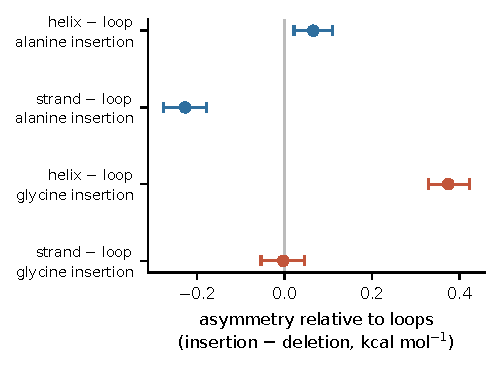
\includegraphics[width=0.58\textwidth]{fig3.pdf}
\caption{\textbf{Switching the inserted residue reverses the helix contrast.} Asymmetry is the
cost of an insertion minus the cost of a deletion at the same position, expressed relative to the
same protein's loops, so that a negative value means the insertion is the cheaper edit there. The
same positions are probed with an alanine and with a glycine insertion. Bars are bootstrap 95\%
intervals over proteins.}
\label{fig:fig3}
\end{figure}

The insertion side of these libraries contains only alanine and glycine, so it supports one
contrast rather than a scale --- but it is a sharp one, because the two residues differ by a
single methyl group and by about 1 kcal\,mol$^{-1}$ of helix propensity \citep{pace1998}. At the
\Nposins{} positions carrying both, the helix--loop contrast in the insertion/deletion asymmetry
is \AlaHL{} $[\AlaHLlo{}, \AlaHLhi{}]$ for alanine and \GlyHL{} $[\GlyHLlo{}, \GlyHLhi{}]$ for
glycine, a shift of about 0.3 kcal\,mol$^{-1}$ from one inserted residue to the other
(Figure~\ref{fig:fig3}). The strand--loop contrast moves from \AlaEL{}
$[\AlaELlo{}, \AlaELhi{}]$ to \GlyEL{} $[\GlyELlo{}, \GlyELhi{}]$, where the glycine interval
contains zero. Restricted to the natural domains alone, the alanine helix contrast is negative
and the glycine one positive, so the two arms differ in sign there; across the full set, which
includes the designed miniproteins, both are positive and it is the size of the contrast rather
than its sign that depends on the inserted residue. We report the full set as primary.

The size of the gap between the two arms is itself informative. Measured directly in the same
data, the difference in cost between inserting glycine and inserting alanine is \GateH{} in
helices, \GateE{} in strands and \GateL{} in loops --- that is, the gap between the two arms of
Figure~\ref{fig:fig3} is the structural preference of alanine over glycine as an inserted residue.
In the designed miniproteins the same switch removes the helix contrast (\DesAlaHL{} to
\DesGlyHL{}).

\subsection{The interaction is real but too small to help prediction}

\begin{figure}[t]
\centering
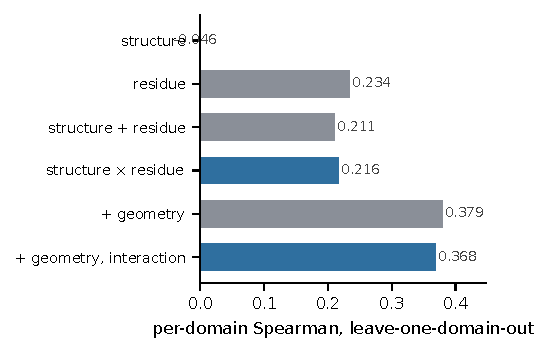
\includegraphics[width=0.58\textwidth]{fig4.pdf}
\caption{\textbf{Leave-one-domain-out prediction of deletion cost.} Ridge models on the same
rows, scored as the mean within-domain Spearman correlation over held-out domains. Adding the
residue-by-structure interaction to the additive model changes little, and once geometric
features are present it does not help at all.}
\label{fig:fig4}
\end{figure}

A statistically unambiguous interaction need not be a useful one. We tested whether modelling it
improves prediction, leave-one-domain-out so that no domain contributes to its own prediction.
It does not. The mean within-domain Spearman correlation rises only from \PredAdd{} for the
additive model to \PredInter{} for the interaction model, a paired gain of \PredGain{}
$[\PredGainLo{}, \PredGainHi{}]$ across \PredNdom{} domains; the interval excludes zero, but the
effect is a fraction of a correlation point and only \PredImproved{} of the domains improve,
barely above chance. Adding relative solvent accessibility, pLDDT and distance to the chain
terminus raises the additive model to \PredGeomAdd{}, and the interaction model is then
\emph{worse} at \PredGeomInt{} (Figure~\ref{fig:fig4}, Table~\ref{tab:pred}).

We report this plainly because it bounds the practical reading of our result. The
residue-by-structure interaction is a real feature of indel energetics, large enough to invalidate
single-number summaries by structural class, and at the same time small relative to the variation
that simple geometric descriptors already capture. Predictors that ignore it are not thereby
losing much accuracy; what they lose is the ability to state a structure-class effect that is
true of all residues.

\subsection{Three negative results}

\paragraph{T4 lysozyme accommodation energies do not transfer.} \citet{vetter1996} determined,
from 32 insertions in nine helices of T4 lysozyme, that bulging within a helix body costs about
4.9 kcal\,mol$^{-1}$ against 2.6 for looping out near a helix end, implying a mid-helix penalty of
roughly 2.3. Across \NhelDom{} domains here the paired within-protein difference between helix
middles and helix ends is \HelMidEnd{} $[\HelMidEndLo{}, \HelMidEndHi{}]$ for alanine insertions.
The direction holds; the magnitude is about five times smaller.

\paragraph{Loop proximity does not govern indel cost.} \citet{heinz1994} described insertions
being absorbed by a register shift that spills residues into the adjacent loop, which predicts
that cost should depend on distance to the nearest loop. Within helices that correlation is
\RhoLoop{} $[\RhoLoopLo{}, \RhoLoopHi{}]$.

\paragraph{Strands are not more indel-tolerant than helices.} Paired within protein, natural
domains appeared to tolerate indels better in strands than in helices (\StrandHelix{}
$[\StrandHelixLo{}, \StrandHelixHi{}]$ for insertions), against the received view, and the effect
survived controls for burial, model confidence, position within the element, residue composition
and an independent structure assignment. It does not replicate in the designed miniproteins
(\DesStrandHelix{} $[\DesStrandHelixLo{}, \DesStrandHelixHi{}]$), and scaled by each protein's
wild-type stability the designed interval excludes the natural estimate. We withdraw it, and
report it because of how it looked before the replication was run.

\section{Discussion}

The field's working summary of indel tolerance --- loops best, helices next, strands worst --- is
an average over a factor that varies more than the summary itself. The deletion data show that
ordering being set by which residue is removed, over a range of roughly 1.3 kcal\,mol$^{-1}$
between the most and least affected residues, and the insertion data show a single methyl group
reversing the sign of the helix--loop comparison.

This has a direct bearing on an existing observation, and the apparent conflict is worth stating
plainly before resolving it. \citet{topolska2025} report that ``the identity of the wildtype aa
only poorly predicts deletion and insertion tolerance'', quantified as a leave-one-domain-out
correlation of $0.226$ for deletions and $0.182$ for insertions from residue identity alone, where
a model built from secondary-structure features reaches $0.538$ and $0.573$. Read at face value
that is the opposite of what we report.

It is not a contradiction, because the two quantities are different. Theirs is the
\emph{marginal} predictive value of residue identity pooled over all structural contexts; ours is
a \emph{within-residue contrast between} structural contexts. A weak marginal is what an
interaction of this shape predicts: if a residue is costly to delete from a helix and cheap from a
loop, its average over contexts carries little information, and the contrast carries it all.
The same arithmetic applies to the small strand-versus-helix differences those authors report;
they are averages over residue identities whose contrasts point in different directions.

The distinction is not merely interpretive. Their predictive models are fitted, in their own
description, ``with lasso regularisation without interaction terms'', so the effect reported here
is one the model could not express.

\paragraph{Why the two arms are needed together.} Each arm has a weakness that the other does not
share, and they are weaknesses of opposite kind. The deletion arm covers all twenty residues, but
the residue at each position was put there by evolution: good helix formers are found in helices
because selection placed them there, so residue and context are not independent, and the
interaction it measures is between a residue and a context it was selected for. The insertion arm
covers only two residues, but alanine and glycine were inserted at every position irrespective of
context, so the assignment is effectively randomised with respect to structure and the
confounding does not arise. The deletion arm therefore supplies the ordering --- which residues
and in what sequence --- while the insertion arm supplies the causal licence for reading that
ordering as an effect of the residue rather than of where evolution put it. Neither is sufficient
on its own.

The periodicity account of \citet{goldman2025} and the register-shift account that goes back to
the T4 lysozyme crystallography \citep{heinz1993,heinz1994,vetter1996} are not contradicted. They
explain why a helix is expensive to edit at all. What they do not predict is the ordering across
residues, which follows helix propensity rather than size and is of the same magnitude as the
mean effect those accounts describe. It is worth noting that the periodicity account has a
difficulty of its own that is independent of anything here: \citet{topolska2025} find the expected
$3$--$4$ residue periodicity in \emph{substitution} tolerance along helices and a two-residue
periodicity along strands, but state that ``neither of these periodicities in variant effects is
observed for insertions or deletions''. The simplest reading is that both operate: backbone geometry
sets the cost of making the edit, and the thermodynamic fit between the residue and its element
sets how much is lost when that particular residue leaves it. That reading also makes the
magnitude of our slope interpretable: helix propensity is defined as the free energy a residue
contributes to helix formation relative to alanine \citep{pace1998}, and a deletion removes that
contribution, so a slope near $-1$ kcal\,mol$^{-1}$ per kcal\,mol$^{-1}$ is what simple
thermodynamic bookkeeping predicts if nothing else changes.

Two findings in the literature bound this picture. \citet{arpino2014} showed that a deletion
inside a GFP helix can be \emph{stabilising}, through a registry shift that repositions a lysine
into a new polar network --- a reminder that the residue term we measure is a population average
over structural responses that are themselves variable. \citet{gutierrez2024} found that
stabilising deletions are enriched at backbone positions under strain, which is a competing source
of context dependence that our analysis does not separate: a residue's propensity and the strain
of the position it occupies are not independent in a natural protein. Resolving the two would need
per-position strain estimates, which we have not computed.

There is one independent line of evidence that the residue matters. \citet{kim2010} analysed short
internal indels between homologous structures and found the residues involved enriched in Gly,
His, Glu, Asp and Ser and depleted in Cys, Phe, Ile, Leu, Trp and Tyr. The residues evolution is
willing to add or remove are, broadly, the ones our measurements say are cheap to remove, and the
aromatic and $\beta$-branched residues it avoids are the expensive ones. This is a qualitative
correspondence between an evolutionary pattern and a thermodynamic one, assembled from separate
studies, and we report it as such rather than as a test.

Practically, the result argues against reporting single-number summaries of indel tolerance by
structural class. It does not argue for adding the interaction to indel effect predictors: the
current indel stability predictor, INDELi, is built from regularised linear models fitted, in its
authors' description, without interaction terms \citep{topolska2025}, and our own test says that
adding one buys almost nothing once geometric features are present. The interaction matters for
how results are described, not for how well they can be predicted.

\paragraph{A note on metrics.} Indel predictors are currently compared across statistics that
cannot be ordered against each other. INDELi reports the mode of per-domain Pearson correlations
on these data, about 0.62 for deletions \citep{topolska2025}, while IFUM reports a pooled Pearson
of 0.80 on a held-out mega-scale set \citep{lee2026}; the ProteinGym indel track averages Spearman
per assay \citep{notin2023}. For the simple structural features used here, pooling across domains
\emph{lowers} the correlation (pLDDT: \PooledR{} pooled against \PerDomR{} per domain), because it
injects between-domain variance in overall indel cost that a within-domain feature cannot explain,
while a model that also predicts domain-level stability gains from that same variance. The
direction of the bias therefore depends on the predictor. Per-protein scoring is the established
convention in variant-effect benchmarking \citep{livesey2025,notin2023}, and both of those sources
caution against comparing correlations across proteins; to our knowledge no equivalent caution has
been stated for indel stability predictors.

\paragraph{Limitations.} All stability measurements come from one assay, protease resistance, in
one deposit. The insertion arm has only two residues; the deletion arm has twenty but the residue
at each position was placed by evolution rather than by design, so the residue and its context are
not independent, and the interaction we report is between a residue and a context in which it was
selected to sit. The strength of the propensity correlation depends on how secondary structure is
assigned: it falls from \RhoPace{} to \SensDep{} when depositor annotations replace ours, though
it stays negative under every assignment we tried. Proline is omitted from the propensity
analysis; the nineteen values we use are
those we could verify, and the analysis is shown in Methods to be insensitive to any value
proline might take. An orthogonal yeast abundance assay on nine domains shows the same ordering of
structure classes but has too few helix positions to test the interaction. The $\beta$-sheet
propensity scales we verified are a weak instrument: two measured at the same position in the
same host agree with each other at \CollinMKSR{} yet give different answers on our contrasts,
and \citet{minorkim1994b} showed that moving the guest site within one protein is enough to
destroy the relationship. We can therefore say that $\beta$ propensity does not predict the
strand contrast better than helix propensity does, but not that the strand arm lacks a
sheet-specific ordering. Settling that needs a sheet propensity scale better than the ones that
exist, or one derived from mega-scale substitution data, which we did not attempt.

\section{Methods}

\paragraph{Data.} Folding stabilities are from \citet{tsuboyama2023}, Zenodo deposit 7992926,
library 3, which contains \NinsTot{} single-residue insertions (alanine and glycine only) and
\NdelTot{} single-residue deletions. For each variant, cost is
$\Delta G_{\mathrm{wt}} - \Delta G_{\mathrm{variant}}$, where $\Delta G_{\mathrm{wt}}$ is the mean
over that construct's wild-type rows. Variants whose reported 95\% confidence interval on
$\Delta G$ exceeds 1 kcal\,mol$^{-1}$ are excluded.

\paragraph{Structure.} Secondary structure was assigned by the hydrogen-bond rules of
\citet{kabsch1983}, implemented directly on the deposited AlphaFold models \citep{jumper2021}:
backbone amide hydrogens placed 1.0\,\AA{} from N opposite the preceding carbonyl, hydrogen bonds
scored by the Kabsch--Sander electrostatic term with a $-0.5$ kcal\,mol$^{-1}$ cutoff, helices
assigned from consecutive $4$-turns, strands from bridge ladders, and elements shorter than five
(helix) or two (strand) residues demoted to loop. The assignment was validated against backbone
geometry that it does not use --- helix residues centre at $\phi = -63.0^\circ$,
$\psi = -41.8^\circ$ with $C\alpha(i)$--$C\alpha(i{+}4) = 6.2$\,\AA{}; strand residues at
$-113.7^\circ$, $+134.1^\circ$ and 12.2\,\AA{} --- and against an independently produced
assignment for the same domains, with which it agrees on \SSagree{} of positions and shows no
helix/strand confusion. Residue numbering was verified against the residue named in each deletion
variant, matching at \NumberMatch{} over \NumberChecks{} variants.

\paragraph{Composition of the set.} Of the \Ndom{} domains analysed, \NNatDom{} are natural,
identified by a PDB accession, and \NDesDom{} are designed: HEEH\_KT and related miniproteins
\citep{rocklin2017} together with trRosetta-hallucinated structures, all from the same deposit.
Every analysis is run on the whole set and again on each part. Designed structures are not a
small adjunct here --- they are \NDesDom{} of \Ndom{} --- so reporting a pooled number alone
would leave the reader unable to tell which population it came from.

\paragraph{Statistics.} Every class comparison is computed within each protein first and then
averaged over proteins, with percentile bootstrap intervals resampling proteins. This is not
cosmetic: a class mean pooled over positions is confounded by protein composition, the
within-versus-between distinction familiar from ecological correlation
\citep{robinson1950,simpson1951,mundlak1978}, and it fails a within-protein permutation control, returning \PooledPerm{} on shuffled data where zero is
expected; the within-protein estimator returns \WithinPerm{} (standard deviation \WithinPermSD{})
over 200 permutations. Regression standard errors are clustered by domain \citep{liang1986,cameron2015} and
confidence intervals resample whole domains \citep{field2007}. Where a difference is examined as
a function of position tolerance, the binning variable is an independent second measurement at the
same position, because binning on one of the two measurements that form a difference produces a
spurious trend \citep{blandaltman1995}; the corresponding regression slope is corrected for
measurement error in the predictor by instrumenting with that second measurement
\citep{hausman2001}. Helix propensities are
the experimental values of \citet{pace1998}; residue volumes are Zamyatnin's; hydropathy is
\citet{kyte1982}.

\paragraph{Proline.} The propensity analysis uses the nineteen values listed in the abstract of
\citet{pace1998}, each checked against that source. Proline is not among them, and we could not
verify a proline value against the paper itself. A figure of 3.16 kcal\,mol$^{-1}$ circulates
attached to this scale; we could not find it in \citet{pace1998}, and note that
\citet{oneil1990} list proline at about 3 on their own helix scale, which is the likely origin
of the number and of its migration between the two. This does not affect the result, for a reason
that can be shown rather than asserted: the correlation is rank-based, and proline ranks last on
every published account of helix propensity, so its numeric value is irrelevant. Giving proline
any value between 1.0 and 5.0 kcal\,mol$^{-1}$ and recomputing moves the correlation only from
\RhoPace{} to between \RhoProLo{} and \RhoProHi{}, and every value at or above 1.5 returns
exactly the same figure.

Proline is nonetheless the one residue that does not follow the trend, and we report this rather
than leave it inside an exclusion. Its measured helix-minus-loop contrast is
$+\ProContrast{}$ kcal\,mol$^{-1}$ over \ProNdom{} proteins, placing it \ProRank{}th of
\ProNranked{} from the most negative end --- near the middle, where the propensity account
predicts it should sit at the extreme alongside glycine (\GlyContrast{}). Deleting a proline from
a helix therefore costs more than the account expects, which is unsurprising given that prolines
in helices sit predominantly at the first turn or at a kink, so removing one is not the same
operation as removing a residue from a regular helical segment. Including proline is the single
largest departure from the reported correlation, and it is in the conservative direction.

\paragraph{Code and data.} All analysis scripts, the pre-registrations written before each test
including those whose marks failed, and the intermediate result files are available at
\url{https://github.com/armixz/indel-cost-residue-not-edit}.

\bibliography{refs}

\clearpage
\appendix
\renewcommand{\thefigure}{S\arabic{figure}}
\renewcommand{\thetable}{S\arabic{table}}
\setcounter{figure}{0}
\setcounter{table}{0}
\section*{Supplementary information}

\begin{table}[t]
\centering
\small
\caption{\textbf{Per-residue deletion contrasts.} For each amino acid, the mean cost of deleting it from a helix minus the mean cost of deleting it from a loop, paired within each protein and averaged over the proteins that contain both. The last two columns split the contrast into its parts, each expressed relative to that protein's own mean deletion cost, showing that the ordering by propensity sits in the helix term. Residues are sorted by helix propensity. Proline is absent: the \citet{pace1998} scale excludes it.}
\label{tab:perres}
\begin{tabular}{llrrrr}
\toprule
Residue & & Helix propensity & Helix $-$ loop & Helix term & Loop term \\
 & & (kcal\,mol$^{-1}$) & (kcal\,mol$^{-1}$) & & \\
\midrule
Ala & A & 0.00 & +0.82 & +0.24 & -0.44 \\
Leu & L & 0.21 & +0.44 & +0.49 & +0.07 \\
Arg & R & 0.21 & +0.67 & +0.18 & -0.33 \\
Met & M & 0.24 & +0.59 & +0.39 & -0.34 \\
Lys & K & 0.26 & +0.82 & +0.08 & -0.67 \\
Gln & Q & 0.39 & +0.64 & +0.01 & -0.68 \\
Glu & E & 0.40 & +0.84 & +0.12 & -0.64 \\
Ile & I & 0.41 & +0.66 & +0.59 & +0.22 \\
Trp & W & 0.49 & +1.12 & +0.60 & +0.39 \\
Ser & S & 0.50 & +0.64 & +0.09 & -0.39 \\
Tyr & Y & 0.53 & +0.33 & +0.45 & +0.05 \\
Phe & F & 0.54 & +0.46 & +0.84 & +0.36 \\
His & H & 0.61 & +0.08 & -0.12 & -0.05 \\
Val & V & 0.61 & +0.51 & +0.39 & +0.07 \\
Asn & N & 0.65 & +0.34 & -0.08 & -0.35 \\
Thr & T & 0.66 & +0.61 & +0.03 & -0.38 \\
Asp & D & 0.69 & +0.22 & -0.12 & -0.21 \\
Gly & G & 1.00 & -0.05 & -0.31 & -0.17 \\
\bottomrule
\end{tabular}
\end{table}


\begin{table}[t]
\centering
\small
\caption{\textbf{Leave-one-domain-out prediction of deletion cost.} Ridge models on the same rows. Each domain is predicted by a model fitted without it. Per-domain Spearman is the mean over held-out domains; the lower decile is reported because a mean can hide a long tail.}
\label{tab:pred}
\begin{tabular}{lrrrr}
\toprule
Model & Features & RMSE & Per-domain $\rho$ & Lower decile \\
\midrule
secondary structure only & 3 & 1.828 & -0.046 & -0.401 \\
residue identity only & 20 & 1.798 & 0.234 & 0.021 \\
structure $+$ residue & 23 & 1.798 & 0.211 & -0.001 \\
structure $\times$ residue & 83 & 1.788 & 0.216 & -0.000 \\
structure $+$ residue $+$ geometry & 26 & 1.683 & 0.379 & 0.081 \\
structure $\times$ residue $+$ geometry & 86 & 1.676 & 0.368 & 0.060 \\
structure $+$ residue $+$ geometry $\times$ structure & 35 & 1.674 & 0.368 & 0.059 \\
\bottomrule
\end{tabular}
\end{table}


\begin{figure}[t]
\centering
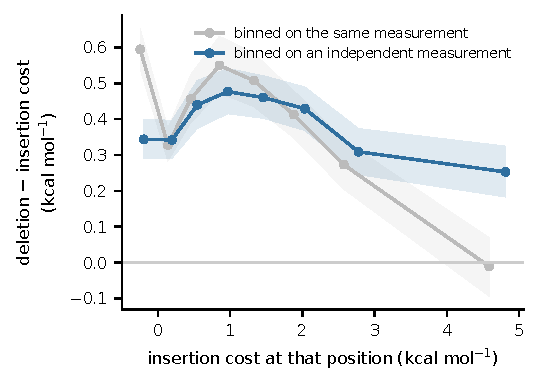
\includegraphics[width=0.56\textwidth]{figS1.pdf}
\caption{\textbf{Binning a difference on one of the measurements that forms it creates a
spurious trend.} The quantity plotted is the deletion cost minus the alanine insertion cost at
the same position. Binning positions on that same alanine insertion cost (grey) makes the
difference appear to fall through zero, because positions with a low measured insertion cost are
enriched for negative measurement error and their independently measured deletion is then higher.
Binning on the glycine insertion at the same position (blue), an independent measurement of the
same tolerance, removes the artefact: the deletion penalty falls by about half across the range
but every bin remains above zero.}
\label{fig:figS1}
\end{figure}

\end{document}
